

%-------------------------------------------------------------------------------
% Dokumenten Klasse
\documentclass[
	final,
	a4paper,
	oneside,
	parskip=full,
	headings=standardclasses,
	headings=big,
	pointednumbers
]{scrartcl}

%-------------------------------------------------------------------------------
% Packete nutzen
\usepackage{ngerman,palatino,setspace}
\usepackage[T1]{fontenc}
\usepackage[utf8]{inputenc}
\usepackage[left=20mm,right=20mm,top=25mm,bottom=25mm]{geometry}
\usepackage{amsmath}
\usepackage{mathtools}
\usepackage{tikz}

\usetikzlibrary{automata, positioning, arrows, calc}

%{
%\tikzset{
%    ->, % makes the edges directed
%    >=stealth, % makes the arrow heads bold
%    node distance=2cm, % specifies the minimum distance between two nodes. Change if necessary.
%    every state/.style={thick, fill=gray!10}, % sets the properties for each ’state’ node
%    every edge/.append style={line width=0.25mm}, % sets the properties for each ’state’ node
%    initial text=$ $, % sets the text that appears on the start arrow
%}
%}

\tikzset{
    node distance=2cm, % Minimum distance between two nodes. Change if necessary.
    every state/.style={ % Sets the properties for each state
        semithick,
        fill=gray!10
    },
    initial text={}, % No label on start arrow
    double distance=2pt, % Adjust appearance of accept states
    every edge/.style={ % Sets the properties for each transition
        draw,
        ->,>=stealth, % Makes edges directed with bold arrowheads
        auto,
        semithick
    },
}


\newcommand{\notaccept}[3]{($(#1)+(#2,#2)$)   -- ($(#1)+(#3,#3)$)
    ($(#1)+(-#2,-#2)$) -- ($(#1)+(-#3,-#3)$)
    ($(#1)+(#2,-#2)$)  -- ($(#1)+(#3,-#3)$)
    ($(#1)+(-#2,#2)$)  -- ($(#1)+(-#3,#3)$)}

%-------------------------------------------------------------------------------
% New Font package
%\usepackage{bm}
%\usepackage[sc]{mathpazo}

\def\boldeps{\boldsymbol{\varepsilon}}

%-------------------------------------------------------------------------------
\usepackage{multirow}

%-------------------------------------------------------------------------------
% uline
\usepackage{ulem}

%-------------------------------------------------------------------------------
% Anderer Font
\usepackage{mathrsfs}
\usepackage[mathcal]{euscript}

%-------------------------------------------------------------------------------
% Square brackets
\usepackage{stmaryrd}

%-------------------------------------------------------------------------------
% Dokument
\begin{document}
    
    \def\pagein{0.15}
    \def\pageout{0.85}
    
    %--- Page 1 --------------------------------------------------------------------
    
    $\Sigma = \left\{ \; a, b \; \right\} $ \quad
    $R = `` \left( \; ab \cup a \; \right)^* "{} $ \quad
    $\mathscr{L} = \llbracket \; \left( \; ab \cup a \; \right)^* \; \rrbracket $
    
    \begin{minipage}{\pagein\textwidth}
        $a$:
    \end{minipage}
    \begin{minipage}{\pageout\textwidth}
        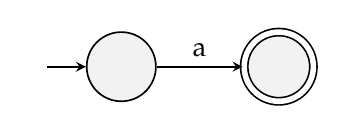
\begin{tikzpicture}
            \node[state, initial left]                  (q1)    {};
            \node[state, accepting, right of=q1]        (q2)    {};
            \draw   (q1) edge[]         node{a} (q2)
            ;
        \end{tikzpicture}
    \end{minipage}
    
    \begin{minipage}{\pagein\textwidth}
        $b$:
    \end{minipage}
    \begin{minipage}{\pageout\textwidth}
        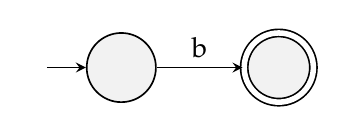
\begin{tikzpicture}
            \node[state, initial left]                  (q1)    {};
            \node[state, accepting, right of=q1]        (q2)    {};
            \draw   (q1) edge[]         node{b} (q2)
            ;
        \end{tikzpicture}
    \end{minipage}
    
    \begin{minipage}{\pagein\textwidth}
        $ab$:
    \end{minipage}
    \begin{minipage}{\pageout\textwidth}
        \def\in{0.25}
        \def\out{0.45}
        \begin{tikzpicture}
            \node[state, initial left]                  (aq1)   {};
            \node[state, accepting, right of=aq1]       (aq2)   {};
            \node[state, right of=aq2]                  (bq1)   {};
            \node[state, accepting, right of=bq1]       (bq2)   {};
            \coordinate (c1) at (aq2);
            \draw   (aq1) edge[]        node{a} (aq2)
                    (bq1) edge[]        node{b} (bq2)
            ;
            \draw[red, thick]
                    ($(c1)+(\in,\in)$)   -- ($(c1)+(\out,\out)$)
                    ($(c1)+(-\in,-\in)$) -- ($(c1)+(-\out,-\out)$)
                    ($(c1)+(\in,-\in)$)  -- ($(c1)+(\out,-\out)$)
                    ($(c1)+(-\in,\in)$)  -- ($(c1)+(-\out,\out)$)
                    (aq2) edge[thick] node{$\boldeps$} (bq1)
            ;
        \end{tikzpicture}
    \end{minipage}
           
    \begin{minipage}{\pagein\textwidth}
       $ab \cup a$:
    \end{minipage}
    \begin{minipage}{\pageout\textwidth}
        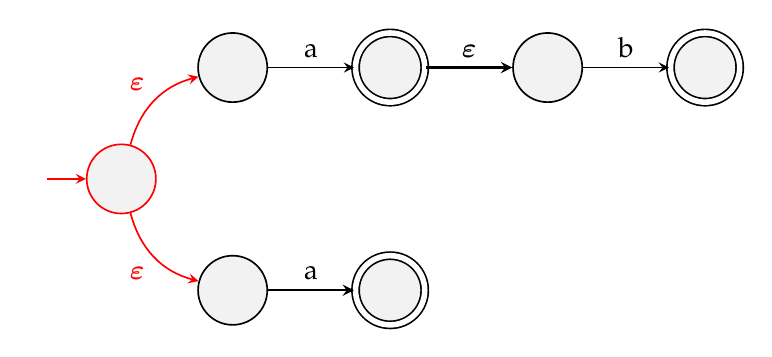
\begin{tikzpicture}[
                every initial by arrow/.style={red}
            ]
            \node[state, initial left, draw=red]                  (aba)   {};
            \node[state, above right of=aba]            (aq1)   {};
            \node[state, accepting, right of=aq1]       (aq2)   {};
            \node[state, right of=aq2]                  (bq1)   {};
            \node[state, accepting, right of=bq1]       (bq2)   {};
            \node[state, below right of=aba]            (aq3)   {};
            \node[state, accepting, right of=aq3]       (aq4)   {};
            \coordinate (x) at (aq2);
            \draw   (aq1) edge[]                        node{a}             (aq2)
                    (bq1) edge[]                        node{b}             (bq2)
                    (aq2) edge[thick]                   node{$\boldeps$} (bq1)
                    (aq3) edge[thick]                   node{a}             (aq4)
            ;
            \draw[red, thick]
                    (aba) edge[bend left]               node{$\boldeps$} (aq1)
                    (aba) edge[bend right, below left]  node{$\boldeps$} (aq3)
            ;
        \end{tikzpicture}
    \end{minipage}
           
    \begin{minipage}{\pagein\textwidth}
       $\left(ab \cup a\right)^*$:
    \end{minipage}
    \begin{minipage}{\pageout\textwidth}
        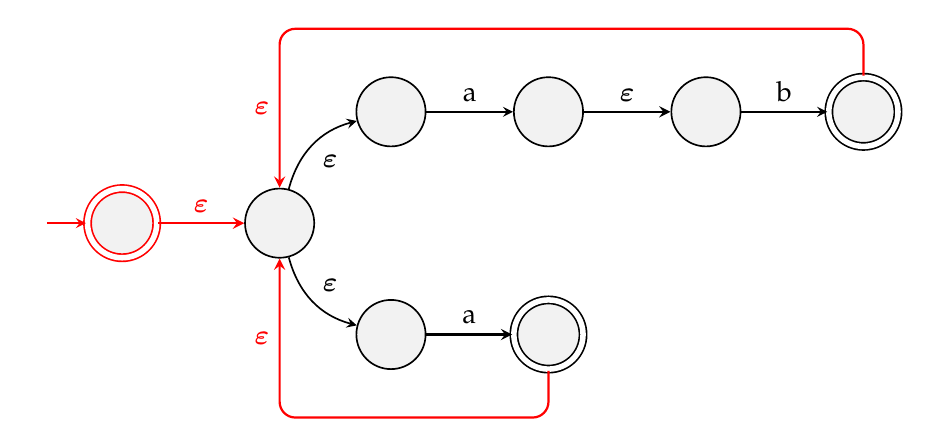
\begin{tikzpicture}[
                every initial by arrow/.style={red}
            ]
            \tikzset{
                rc/.style={->,>=stealth,red,thick,rounded corners=2mm}
            }
            \node[state,initial left,accepting,draw=red](start) {};
            \node[state, right of=start]                (aba)   {};
            \node[state, above right of=aba]            (aq1)   {};
            \node[state, right of=aq1]       (aq2)   {};
            \node[state, right of=aq2]                  (bq1)   {};
            \node[state, accepting, right of=bq1]       (bq2)   {};
            \node[state, below right of=aba]            (aq3)   {};
            \node[state, accepting, right of=aq3]       (aq4)   {};
            \coordinate (x) at (bq2);
            \draw   (aq1) edge[]                        node{a}             (aq2)
                    (bq1) edge[]                        node{b}             (bq2)
                    (aq2) edge[thick]                   node{$\boldeps$}    (bq1)
                    (aq3) edge[thick]                   node{a}             (aq4)
                    (aba) edge[bend left,  below right] node{$\boldeps$}    (aq1)
                    (aba) edge[bend right, above right] node{$\boldeps$}    (aq3)
            ;
            %\draw[step=1cm,gray,very thin]
            %        (0, -3) grid (10,3);
            %;
            \draw[red,thick]
                    (start) edge[thick]                 node{$\boldeps$}    (aba);

            \draw[rc]
                    let \p1 = (bq2),
                        \p2 = (aba)
                    in
                    (bq2) -- (\x1, \y1+30) -- (\x2,\y1+30) -- node[left]{$\boldeps$} (aba);
            \draw[rc]
                    let \p1 = (aq4),
                        \p2 = (aba)
                    in
                    (aq4) -- (\x1, \y1-30) -- (\x2,\y1-30) -- node[left]{$\boldeps$} (aba);
                    
            ;
            %\draw[->,>=stealth,red,thick]
            %        (bq2) .. controls (8,3)
            %                    and      (1,4) ..   node[yshift=-0.3cm]{$\boldeps$} (aba)
            %        (aq4) .. controls (5,-3)
            %                    and      (1,-3) ..  node[yshift=0.3cm]{$\boldeps$} (aba)
            %;
        \end{tikzpicture}
    \end{minipage}
    
    $\Sigma = \left\{ \; 0, 1 \; \right\} $ \quad
    $R = `` \left( \; 0 \cup 1 \; \right)^* 10 "{} $ \quad
    $\mathscr{L} = \llbracket \; \left( \; 0 \cup 1 \; \right)^* 10 \; \rrbracket $
           
    \begin{minipage}{\pagein\textwidth}
       $\left(ab \cup a\right)^*$:
    \end{minipage}
    \begin{minipage}{\pageout\textwidth}
        \def\in{0.25}
        \def\out{0.45}
        \begin{tikzpicture}
            \tikzset{
                rc/.style={->,>=stealth,thick,rounded corners=2mm}
            }
            \node[state,initial left,accepting]         (start) {};
            \node[state, right of=start]                (01)    {};
            \node[state, above right of=01]             (0q1)   {};
            \node[state, accepting, right of=0q1]       (0q2)   {};
            \node[state, below right of=01]             (1q1)   {};
            \node[state, accepting, right of=1q1]       (1q2)   {};
            \coordinate (c1) at (0q2);
            \coordinate (c2) at (1q2);
            %\coordinate (c3) at (aq2);
            \draw   (0q1) edge[]                        node{0}             (0q2)
                    (1q1) edge[]                        node{1}             (1q2)
                    (01) edge[bend left,  below right]  node{$\boldeps$}     (0q1)
                    (01) edge[bend right, above right]  node{$\boldeps$}     (1q1)
                    (start) edge[thick]                 node{$\boldeps$}    (aba)
            ;

            \draw[rc]
                    let \p1 = (0q2),
                        \p2 = (01)
                    in
                    (0q2) -- (\x1, \y1+22) -- (\x2,\y1+22) -- node[left]{$\boldeps$} (01);
            \draw[rc]
                    let \p1 = (1q2),
                        \p2 = (01)
                    in
                    (1q2) -- (\x1, \y1-22) -- (\x2,\y1-22) -- node[left]{$\boldeps$} (01);
                    
            ;
            \draw[thick]
                    ($(c1)+(\in,\in)$)   -- ($(c1)+(\out,\out)$)
                    ($(c1)+(-\in,-\in)$) -- ($(c1)+(-\out,-\out)$)
                    ($(c1)+(\in,-\in)$)  -- ($(c1)+(\out,-\out)$)
                    ($(c1)+(-\in,\in)$)  -- ($(c1)+(-\out,\out)$)
                    \notaccept{c2}{\in}{\out}
                    (aq2) edge[thick] node{$\boldeps$} (bq1)
            ;
            %\draw[->,>=stealth,red,thick]
            %        (bq2) .. controls (8,3)
            %                    and      (1,4) ..   node[yshift=-0.3cm]{$\boldeps$} (aba)
            %        (aq4) .. controls (5,-3)
            %                    and      (1,-3) ..  node[yshift=0.3cm]{$\boldeps$} (aba)
            %;
        \end{tikzpicture}
    \end{minipage}
    
    %--- Page 2 --------------------------------------------------------------------
    \newpage    

    

    %--- Page 3 --------------------------------------------------------------------
    \newpage

	
    %--- Page 4 --------------------------------------------------------------------
    \newpage
    


    %--- Page 5 --------------------------------------------------------------------
    \newpage
    
    

    %--- Page 6 --------------------------------------------------------------------
    \newpage


\end{document}
